%!TEX root = ../paper.tex

\begin{sidewaysfigure*}
{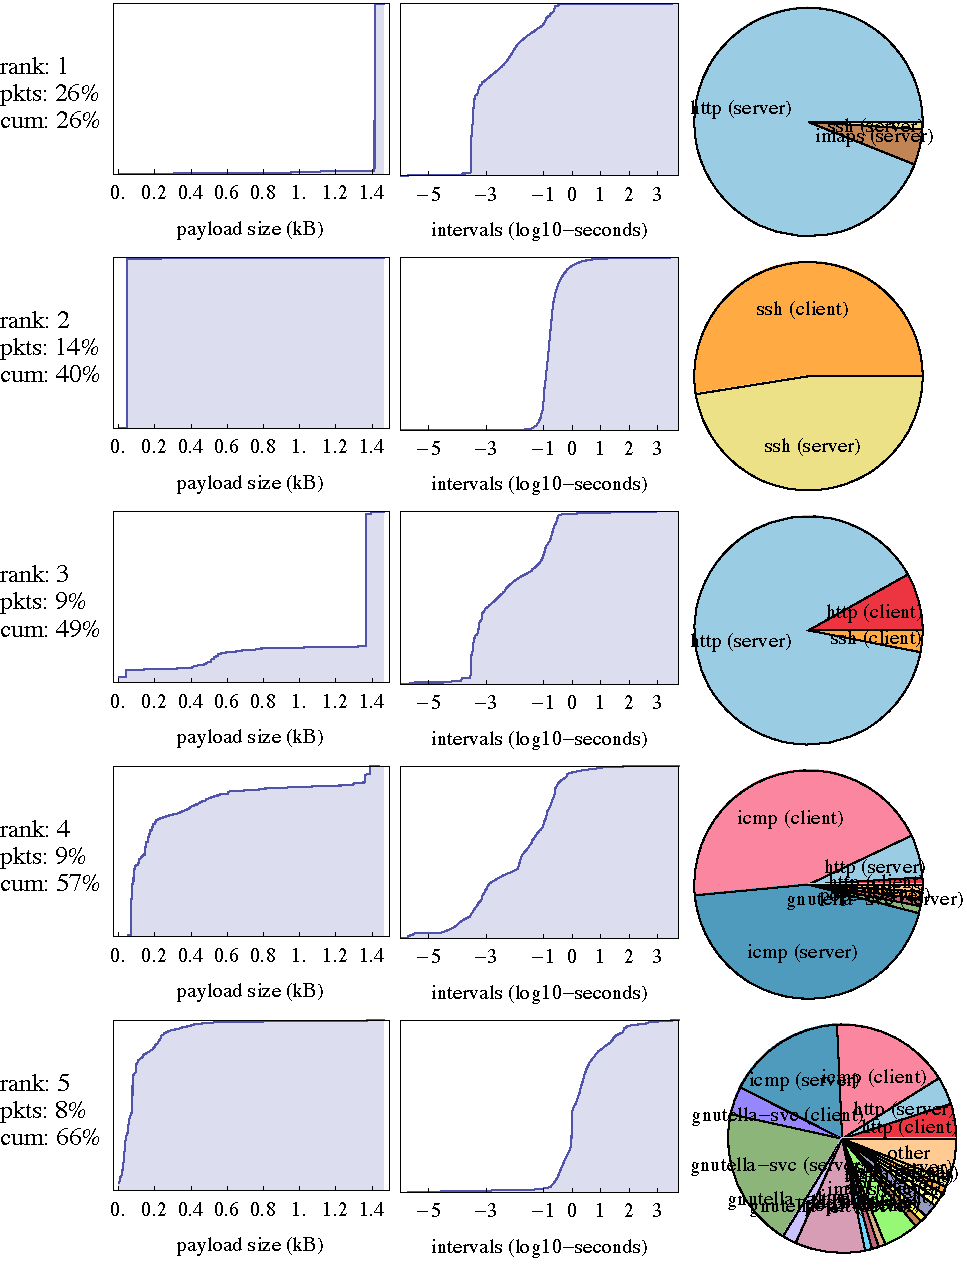
\includegraphics[height=5.95in]{basic_behaviors_1.pdf}}\hfill%
{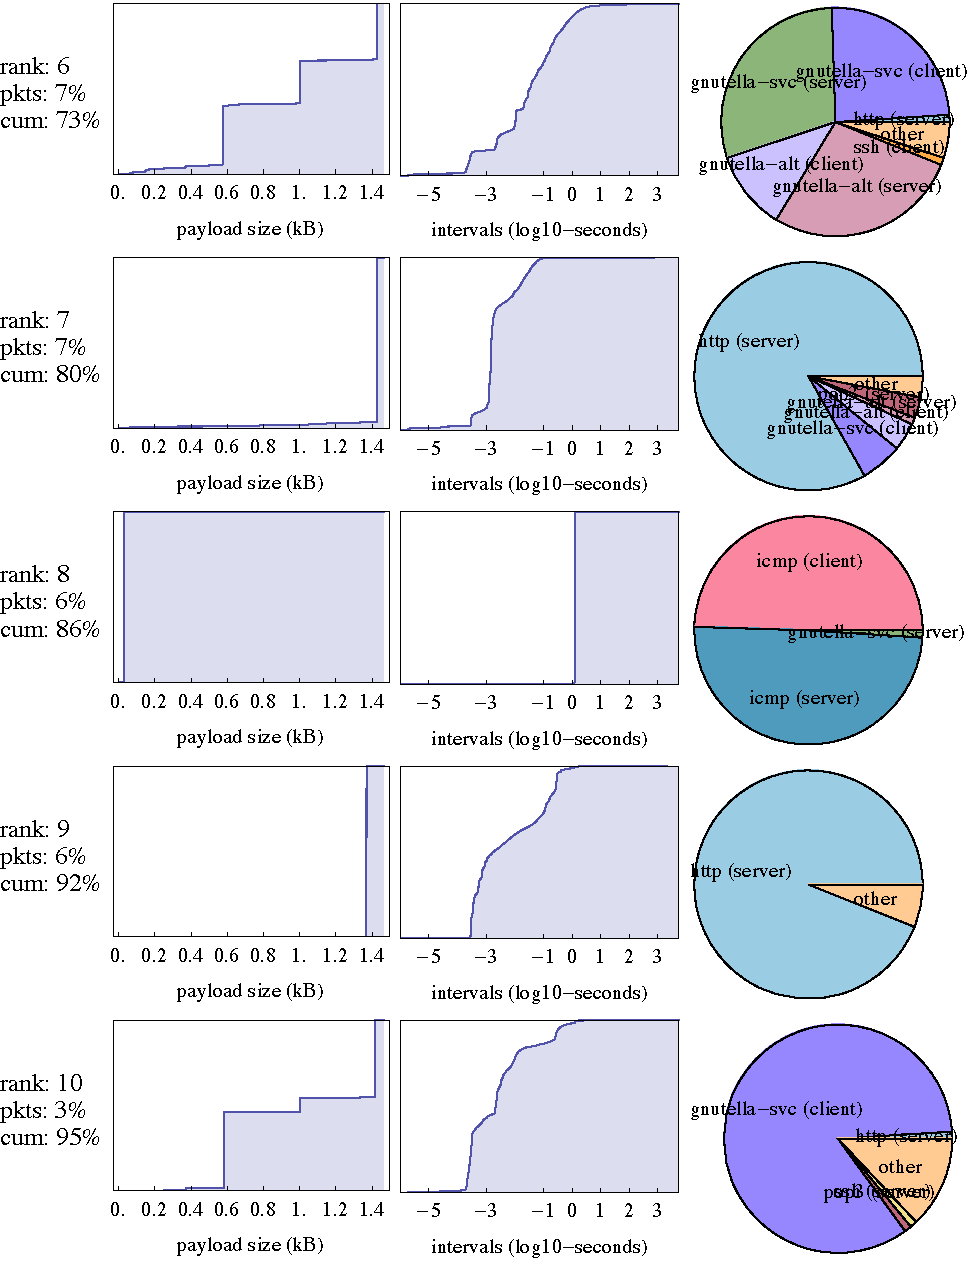
\includegraphics[height=5.95in]{basic_behaviors_2.pdf}}
\caption{%
The ten most prevalent components of flow behavior as pairs of packet payload size and of inter-packet interval distributions.
The distributions are shown as cumulative distribution functions: the $x$-axis represents payload size (in kilobytes) or inter-packet interval duration (in log-seconds, base 10), respectively;
the $y$-axis indicates the probability a value occurring, less than or equal to the $x$ value.
The behaviors are ordered in descending rank of how many packets they explain;
to the left, each behavior's rank is indicated, together with the percentage of total packets associated with it, and the cumulative percentage of packets explained.
To the right of each behavior is a pie chart showing the breakdown of associated packets by protocol, as determined by well-known port numbers.
Pie slices are only labeled if they constitute at least 3\% of associated packets.
}
\label{fig:basic-behaviors}
\end{sidewaysfigure*}
